%% 歩容パターンの再評価手法の提案.tex
%% LaTeX-2e 専用

%% 全体の流れとしては,まず,先行研究の問題点を指摘し,次に,歩容パターンの再評価手法を提案する.

\chapter{歩容パターンの再評価手法の提案}\label{chapter:歩容パターンの再評価手法の提案}
第\ref{chapter:歩容パターンの再評価手法の提案}章では,先行研究の手法およびその問題点を指摘し,
常に脚軌道生成が可能な自由歩容パターン生成手法として,歩容パターンの再評価手法を述べる.

% 先行研究の章
\section{本研究室における自由歩容パターン生成の先行研究}
最初にグラフ探索よる自由歩容パターン生成手法において用いる用語を定義し,
先行研究で行われてきた自由歩容パターン生成手法について述べる.
また,先行研究で用いられてきた自由歩容パターン生成手法の問題点について述べる.

\subsection{グラフ理論について}
本論文ではグラフ理論を用いた自由歩容パターン生成手法を論ずるため,まずはグラフ理論について説明をする.
グラフとは,頂点(ノード)とそれらを結ぶ辺(エッジ)からなる図形である.
このグラフを用いて,さまざまな問題を取り扱う学問をグラフ理論という.

以降の説明を簡単にするため,この論文で用いるグラフ理論の用語について簡潔に述べる.
グラフ上のあるノードから別のノードにエッジを用いて移動することを遷移と呼ぶ.
遷移の際,移動前のノードを始点,移動後のノードを終点と呼ぶ.
グラフの種類は大別して有向グラフと無向グラフに分けられ,
エッジに向きがあるものを有向グラフ(\figref{fig:directed_graph}),
逆に向きを持たないものを無向グラフ(\figref{fig:undirected_graph})という.
また,閉路を持たず,かつ,すべてのノード間にエッジが存在するグラフを木という.
このような木構造をもつグラフのうち,\figref{fig:tree_graph}のように,
根となるノードを持ち,そのノードからすべてのノードに到達可能なものを根付き木という.
根付き木を図形として表現する場合は簡単のため,
\figref{fig:tree_graph}のように根を上部に配置することが多い.

根付き木には無向グラフと有向グラフの2種類が存在するが,
後述する歩行パターングラフは有効グラフであるため,
有向の根付き木について説明を行う.
根付き木のエッジが,根が始点となるように伸びている場合,
あるノードから遷移可能なノードをそのノードの子ノードと呼ぶ.
逆に,あるノードに遷移可能なノードをそのノードの親ノードと呼ぶ.
親ノードを持たないノードを根ノードと呼び,子ノードを持たないノードを葉ノードと呼ぶ.
また,あるノードから根ノードまでのエッジの数をそのノードの深さと呼び,
根ノード自身の深さは0となる.

例えば\figref{fig:tree_graph}において,ノードAが根ノードであり,ノードB,Cがその子ノードである.
また,ノードB,ノードD,E,ノードCはノードFを子ノードとして持ち,ノードD,E,Fは葉ノードである.
ノードAの深さは0であり,ノードB,Cの深さは1,ノードD,E,Fの深さは2となる.

\begin{figure}[h]
  \subfigure[Undirected Graph]{%
  \label{fig:undirected_graph}
  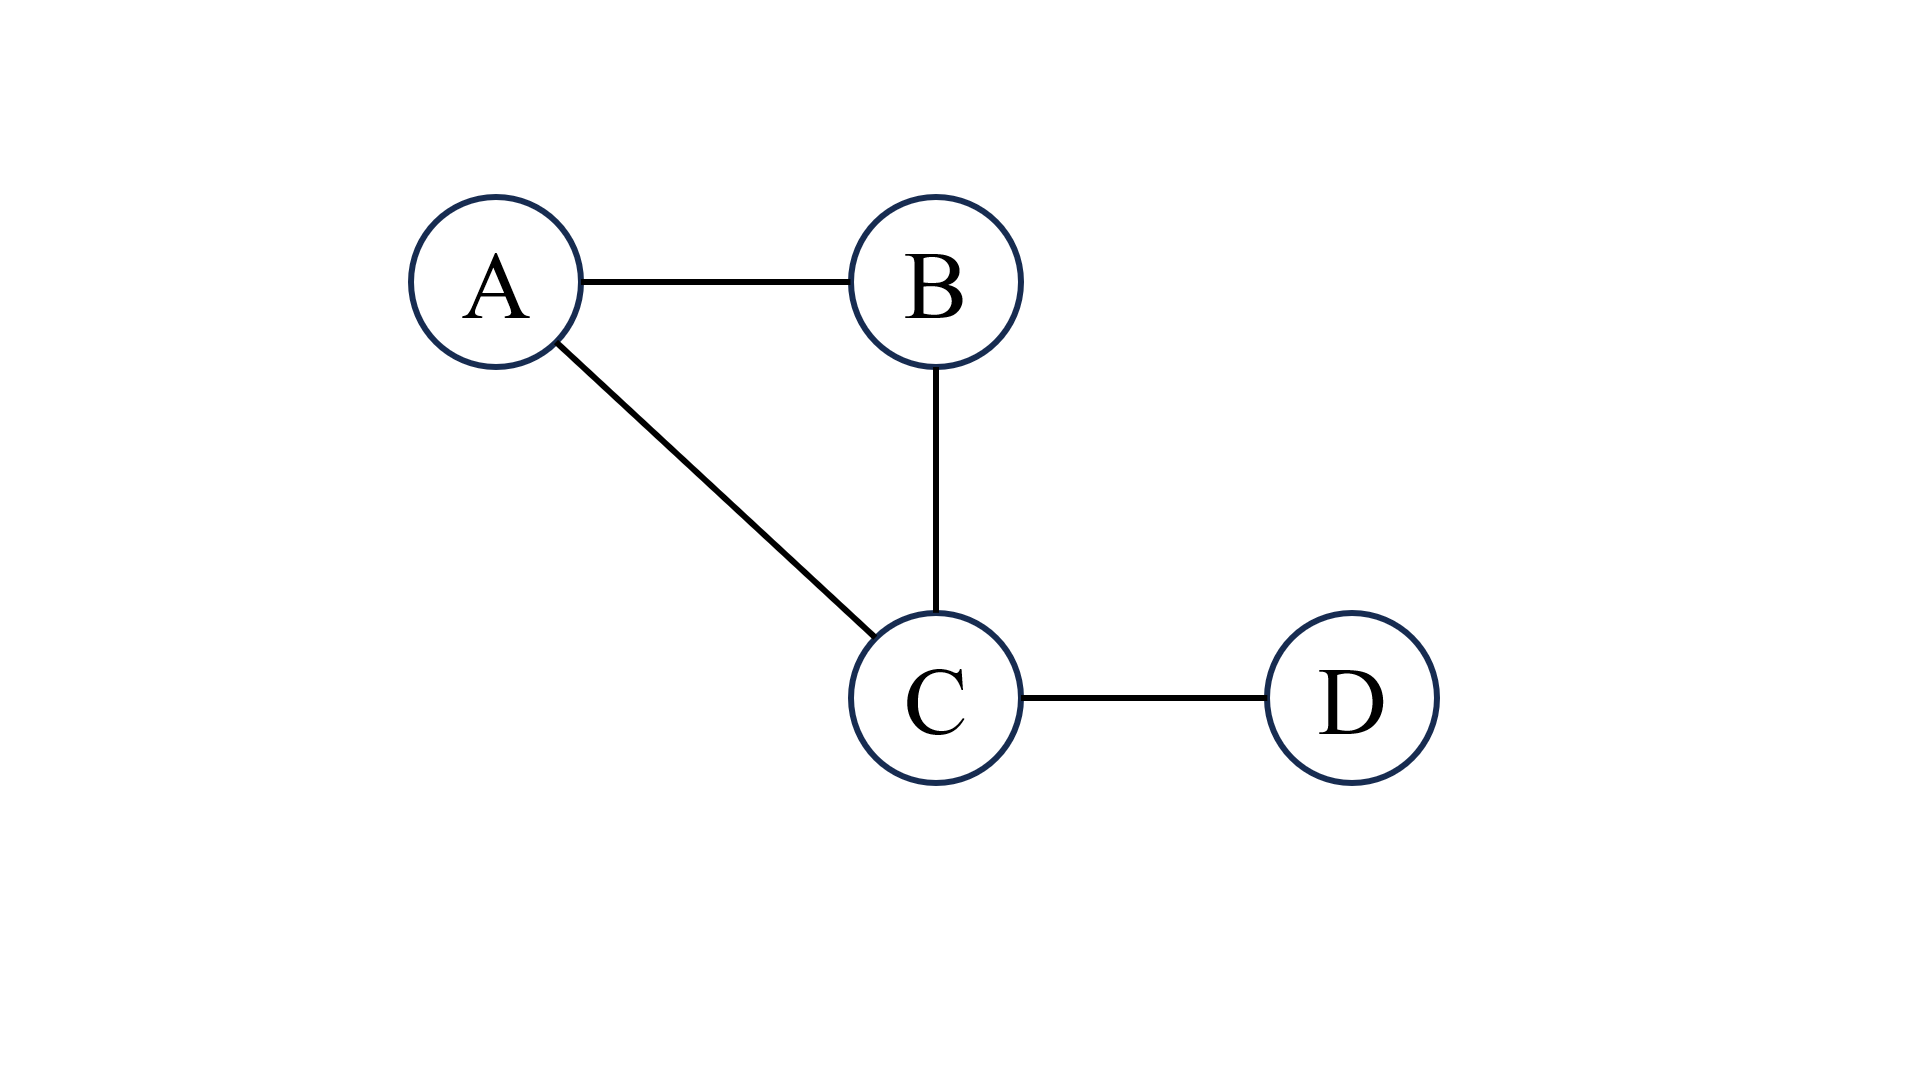
\includegraphics[width=0.48\columnwidth]{figure/chapter2/undirected_graph.png}}
  \hspace{0.04\columnwidth}
  \subfigure[Directed Graph]{%
  \label{fig:directed_graph}
  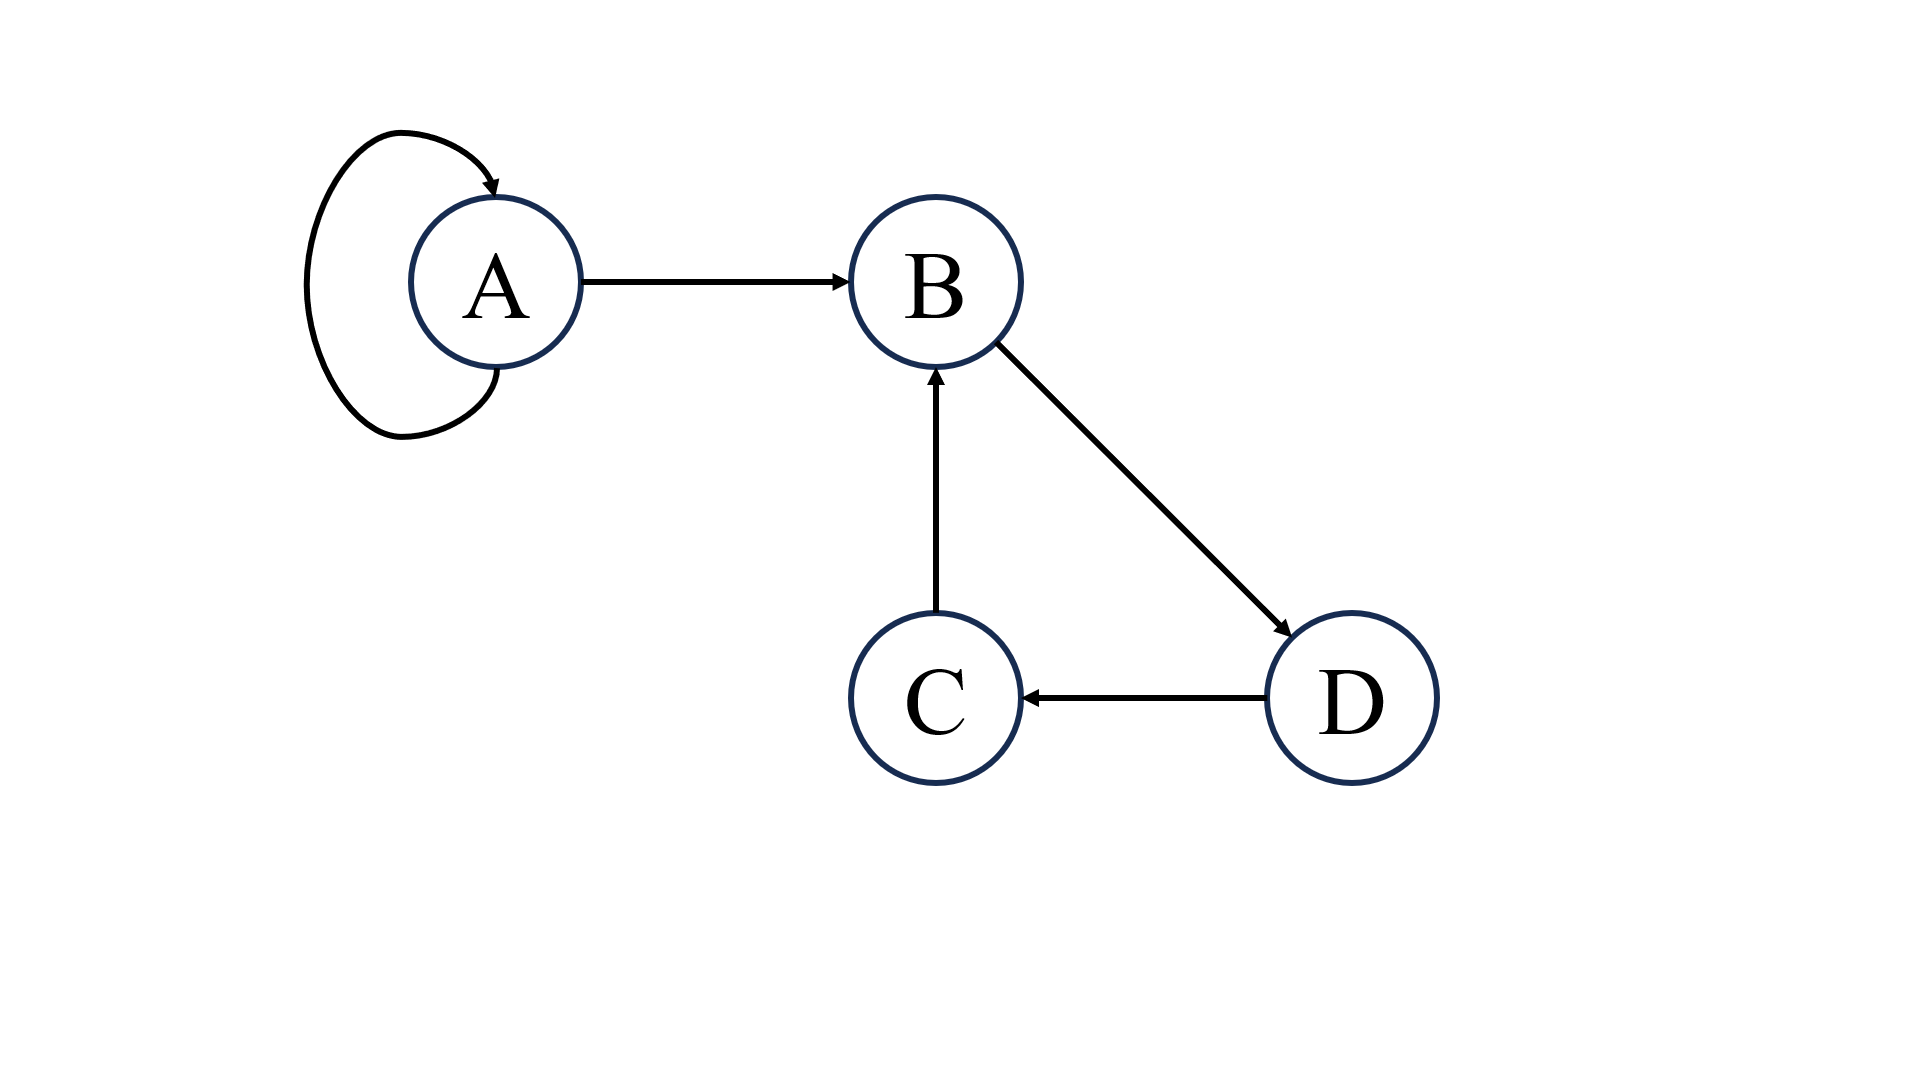
\includegraphics[width=0.48\columnwidth]{figure/chapter2/directed_graph.png}}
  \caption{Examples of simple graphs}
  \label{fig:example_simple_graphs}
\end{figure}

\begin{figure}[h]
  \begin{center}
    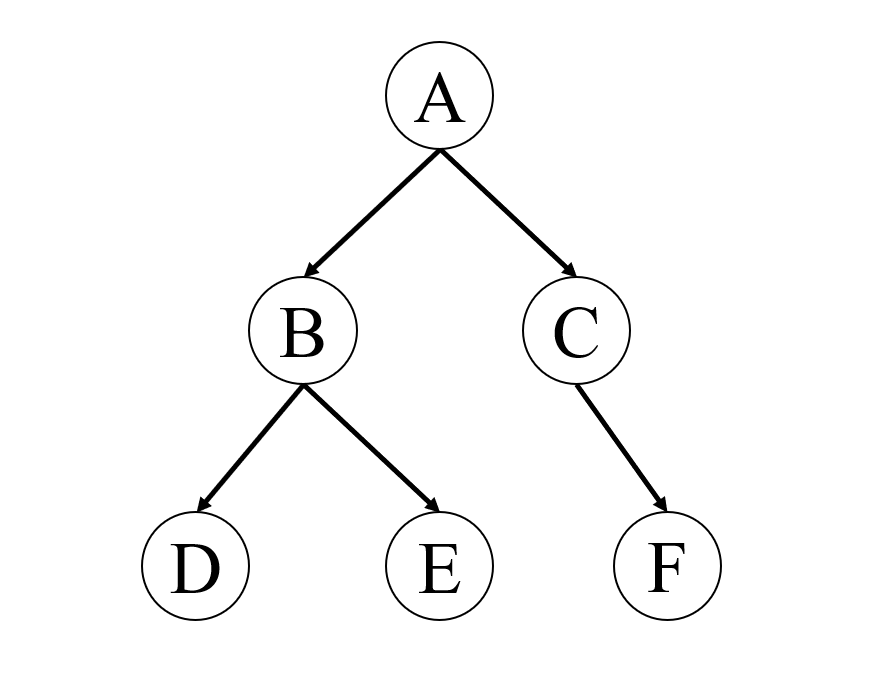
\includegraphics[width=50mm, clip]{figure/chapter2/tree_graph.png}
    \caption{Tree Graph}
    \label{fig:tree_graph} % chktex 24
  \end{center}
\end{figure}

グラフのあるノードから別のノードに到達するための経路をパスと呼び,
これを求めることをグラフ探索と呼ぶ.
グラフ探索には,深さ優先探索,幅優先探索などのさまざまなアルゴリズムが存在する.
深さ優先探索では,始点となるノードから,深さが深くなる方向を優先して探索を行う.
これに対して,幅優先探索では,始点となるノードから,深さが浅いノードを優先して探索を行う手法である.

\subsection{歩容パターングラフの定義}
本研究においては,6脚ロボットの歩容パターンをグラフを用いて表現する.
グラフはロボットの状態をノードとし,ロボットの状態間の遷移,つまりロボットの動作をエッジとして作成する.
グラフは有向の根付き木とし,現在のロボットの状態を根ノード,
その姿勢から1動作で到達できる姿勢を子ノードとして根ノードに接続する.
また,このようにして作られたグラフを歩容パターングラフと定義する.

本手法では,まず歩容パターングラフを作成する.
そして,根ノードから最も最適な動作を行う葉ノードまでのパスを,グラフ探索によって求め,
そのパスに含まれる深さ1のノードを次の動作としてロボットに実行させる.
これを繰り返すことで,ロボットの歩容パターンを生成しているのである.

グラフ探索による歩容パターン生成においては,網羅的にロボットの状態を調べ上げるため,
実時間内の計算を行うにはグラフの規模を小さくすることが求められる.
しかし,歩容パターングラフはロボットの状態や動作を対象とするため無数の組み合わせが存在し,
そのすべてを網羅的に調べ上げることは困難である.
そのため,状態や動作を離散化することで歩容パターン生成をグラフへ落とし込む必要がある.
以下に各要素の離散化について述べる.

\subsubsection{グラフの階層構造}
前述のとおり,ロボットの脚位置は脚の可動範囲内であれば,無数の位置を取ることができる.
そのため本手法では,基準となる脚位置を決め,その基準からの相対位置を用いて脚位置を離散化している.
Prabirらが提案した手法では2次元平面での移動を前提としていたが\cite{Prabir_Graph_search},
これを三浦が3次元空間へ拡張した\cite{Miura_Graph_search}.

\figref{fig:discretization}に支持脚の脚位置の離散化の様子を示した.
\figref{fig:discretization}のように脚位置の基準座標を4とし,
脚位置4と同じ高さにあるかつ,進行方向に対して基準位置よりも前方にある脚位置を6,後方にある脚位置を2とする.
また,脚位置6よりも高い位置にある脚位置を7,低い位置にある脚位置を5とし,
脚位置2よりも高い位置にある脚位置を3,低い位置にある脚位置を1とする.
このようにして,脚位置を7つに離散化している.
遊脚している脚の脚位置は,支持脚の脚位置1$\sim$7に対応させ,脚位置1'$\sim$7'とする.% $\sim$ で波線を引く

これにより,脚位置1$\sim$7から脚位置1'$\sim$7'への遷移によって,脚の上下運動を表現することができる.
また,脚位置1'$\sim$7'内での遷移によって,遊脚の水平方向の移動を表現することができる.
以上より,脚の上下運動と脚の水平方向の移動をグラフで表現することができることを示した.

\begin{figure}[h]
  \begin{center}
    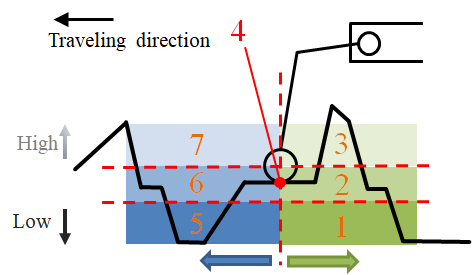
\includegraphics[width=75mm, clip]{figure/chapter2/discretization_of_leg_pos.png}
    \caption{Discretization of Leg Posistion}
    \label{fig:discretization} % chktex 24
  \end{center}
\end{figure}

このような脚位置の離散化を行うことで,脚位置の組み合わせを有限個に抑えることができるが,
脚位置の組み合わせは未だ,$7^6 = 117649 \approx 10^5$通り存在し,
遊脚である時を含めるとさらに組み合わせが増えることがわかる.
プログラムの実行環境によって左右されるが,
プログラミング言語のC++で作成した処理では約1秒間に$10^8$回程度の計算が可能であるとされており\cite{Program_Challenge_Book},
この組み合わせをすべて歩容パターングラフに追加した場合,実時間内の処理を行うにはグラフの規模が大きくなりすぎる.
そこで,大木らは脚位置の組み合わせを階層構造化することで,
遊脚時の脚位置1'$\sim$7'を省略し,探索するノード数を減らすことに成功した\cite{Oki_Graph_search}.

階層構造とこれを利用した探索の方法を説明するために,遊脚の組み合わせと脚位置の組み合わせについて定義を行う.
遊脚の組み合わせは,ロボットの各脚について,その脚が遊脚であるか支持脚であるかを表すノードの要素である.
6脚ロボットの右前脚を1番目の脚として,時計回りに2番目の脚から6番目の脚とする.
この時,i番目の脚が支持脚であることを$v_i = 1$,遊脚である時を$v_i = 0$とすると,
遊脚の組み合わせ$V$は\eqref{eq:leg_com}のように表すことができる.

\begin{equation}\label{eq:leg_com}
  V = \{v_1, v_2, v_3, v_4, v_5, v_6\}
\end{equation}

\noindent 遊脚の組み合わせは$2^6 = 64$通り存在するが,
6脚,5脚,4脚が遊脚である組み合わせや,
隣り合う3脚が遊脚である組み合わせは
実際には取りえない組み合わせであるため,
探索するべき組み合わせは$2^6 - {}_6 \mathrm{C}_6 - {}_6 \mathrm{C}_5 - {}_6 \mathrm{C}_4 - 6 = 36$通りとなる.

また,脚位置の組み合わせとは離散化した脚位置において,各脚がどの位置にあるかを表すノードの要素である.
i番目の脚が脚位置jにあることを$k_i = j$とすると,
脚位置の組み合わせ$K$は\eqref{eq:leg_pos}のように表すことができる.

\begin{equation}\label{eq:leg_pos}
  K = \{k_1, k_2, k_3, k_4, k_5, k_6\}
\end{equation}

\noindent\eqref{eq:leg_com},\eqref{eq:leg_pos}より
ロボットの脚の状態は遊脚の組み合わせ$V$と脚位置の組み合わせ$K$を用いて表すことができるようになった.
i番目の脚の状態を$l_i = v_i \cdot k_i$とすると,$L$は\eqref{eq:leg_state}のように表すことができる.

\begin{equation}\label{eq:leg_state}
  L_{ij} = \{v_1 \cdot k_1, v_2 \cdot k_2, v_3 \cdot k_3, v_4 \cdot k_4, v_5 \cdot k_5, v_6 \cdot k_6\}
\end{equation}

\noindent\eqref{eq:leg_state}より,脚位置の組み合わせが$K = \{1,1,1,1,1,1\}$で
遊脚の組み合わせが$V = \{0,1,0,1,0,1\}$である時の脚の状態を$L_{ij} = \{0,1,0,1,0,1\}$と表すことができる.
同様に,脚位置の組み合わせが$K = \{3,1,3,1,3,1\}$で遊脚の組み合わせが$V = \{0,1,0,1,0,1\}$である時の脚状態は
$L_{ij} = \{0,1,0,1,0,1\}$と表すことができる.
このことから,ある脚位置の組み合わせから,別の脚位置の組み合わせへの遷移は,
脚の状態$L$が等しいときのみ可能であることがわかる.

以上の定義より,階層構造と探索方法について説明することができる.
階層とは脚位置の組み合わせ$K$が等しく,かつ,遊脚の組み合わせ$V$が異なるノードの集合と定義され,
遊脚の組み合わせが36通り存在することから,同じ階層内のノードは36個存在する.
脚の上下運動を実現したい場合は,遊脚の組み合わせ$V$が異なるノードを探索する必要があるため,
図\ref{fig:hierarchy2}のように階層内のノード36個のみを探索すればよい.

また,脚の水平運動を実現したい場合は,脚位置の組み合わせ$K$が異なるノードを探索する必要があるため,
図\ref{fig:hierarchy}のように脚の状態$L$が等しくなるノードのみを探索すればよい.
脚の状態$L$が等しくなるノードは,最大で3脚が遊脚しているときの$7^3 = 343$個であるため,
十分に実時間内の計算が可能である.

\begin{figure}[htbp]
  \begin{center}
    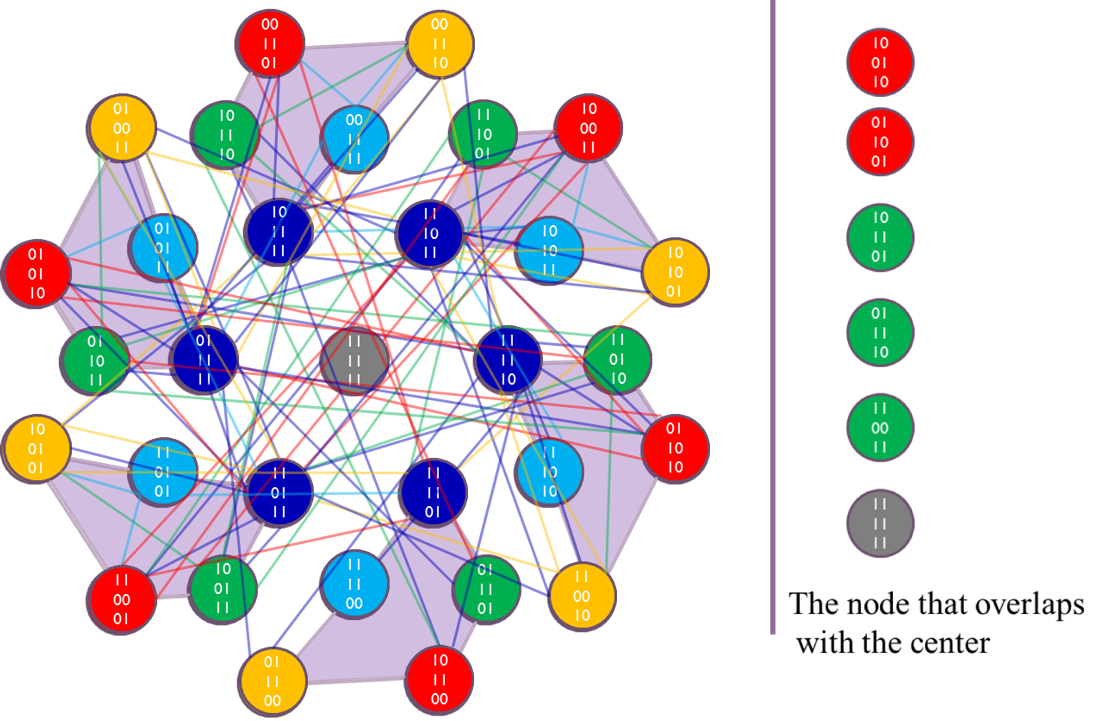
\includegraphics[width=75mm, clip]{figure/chapter2/hierarchy2.png}
    \caption{Search in the Same Hierarchy}
    \label{fig:hierarchy2} % chktex 24
  \end{center}
\end{figure}

\begin{figure}[htbp]
  \begin{center}
    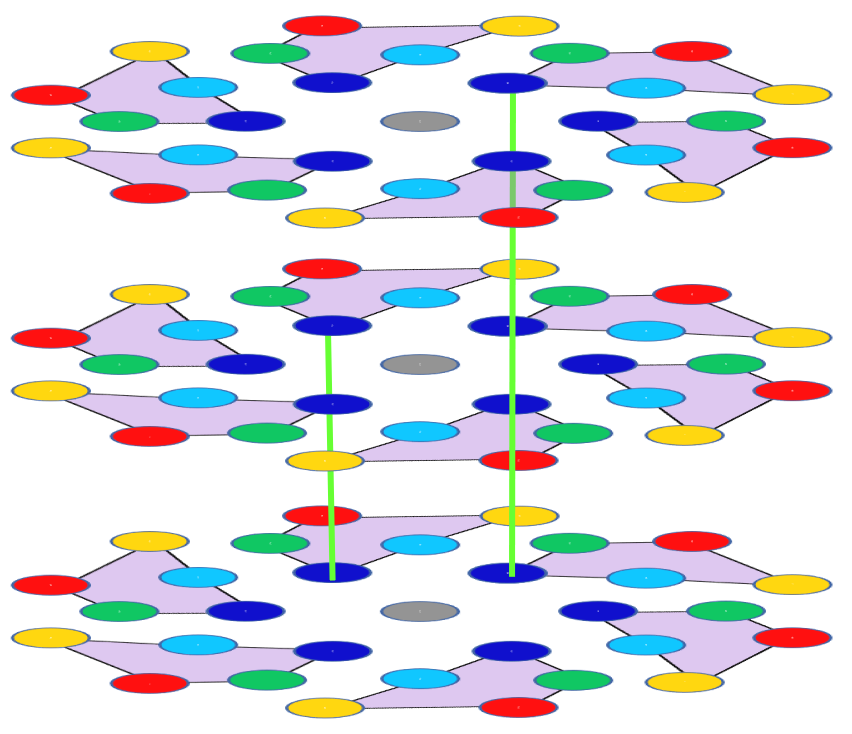
\includegraphics[width=75mm, clip]{figure/chapter2/hierarchy.png}
    \caption{Search in the Difficult Hierarchy}
    \label{fig:hierarchy} % chktex 24
  \end{center}
\end{figure}

\subsubsection{脚軌道生成の分離}
次に歩容パターングラフのエッジについて述べる.
歩容パターングラフにおいて,エッジはロボットの動作を表す.
ロボットの動作は脚の接地・遊脚運動と,重心の移動からなるため,これらの動作に対応するエッジを作成する.
具体的には,脚の上下移動のエッジ,脚の水平移動のエッジ,重心の上下移動のエッジ,
重心の水平移動のエッジ,そして,重心の回転のエッジを用いてロボットの動作を表現する.

これらのエッジには,移動前と移動後のノードを補完するための状態を持っておらず,
単純に移動前と移動後のノードを結ぶのみである.
これはつまり,歩容パターングラフを生成するプログラムと,脚軌道を生成するプログラムが分離されていることを意味する.
脚軌道を考える場合,ロボットの関節の可動範囲を考慮する必要があり,逆運動学解を用いる脚の関節角度の計算が求められる.
しかし,逆運動学の計算には計算負荷の大きい逆三角関数の計算が必要となり,各エッジについて網羅的に計算を行うことを考えると,
実時間内の計算が困難になってしまう.
そのため本手法では,歩容パターングラフを生成するプログラムを分離し,
歩容パターングラフの生成時には脚の可動範囲は近似的な値を用いて計算することで,
実時間内の計算を可能にしている.

近似的な脚の可動範囲の求め方について述べる.
近似的な脚の可動範囲は脚の付け根を中心とする環状の扇形として表現する.
簡単のため,以降は扇形の外径を最大半径,内径を最小半径と呼ぶことにする.
まず,脚先が届くことができる範囲を求めるために,最大半径を以下の手順で求める.
\begin{enumerate}
  \item 図\ref{fig:leg_range_a}のように水平方向に脚先を$1 [mm]$ずつ伸ばす.
  \item 脚先を伸ばすことができなくなった場合,\\
        図\ref{fig:leg_range_b}のように脚先と脚の付け根の高さ方向の距離の差をインデックスとして,\\
        脚先と第1関節の水平方向の距離を最大半径として記録する.
  \item 脚先を$1 [mm]$下げて同様の処理を繰り返す.脚先を下げることができなくなった場合,処理を終了する.
\end{enumerate}
次に最小半径をロボットの脚長などのパラメータから決定する.
先行研究では実験機にあわせ,$120 [mm]$とした.

\begin{figure}[h]
  \subfigure[Horizontal Movement of the Leg Tips]{%
  \label{fig:leg_range_a}
  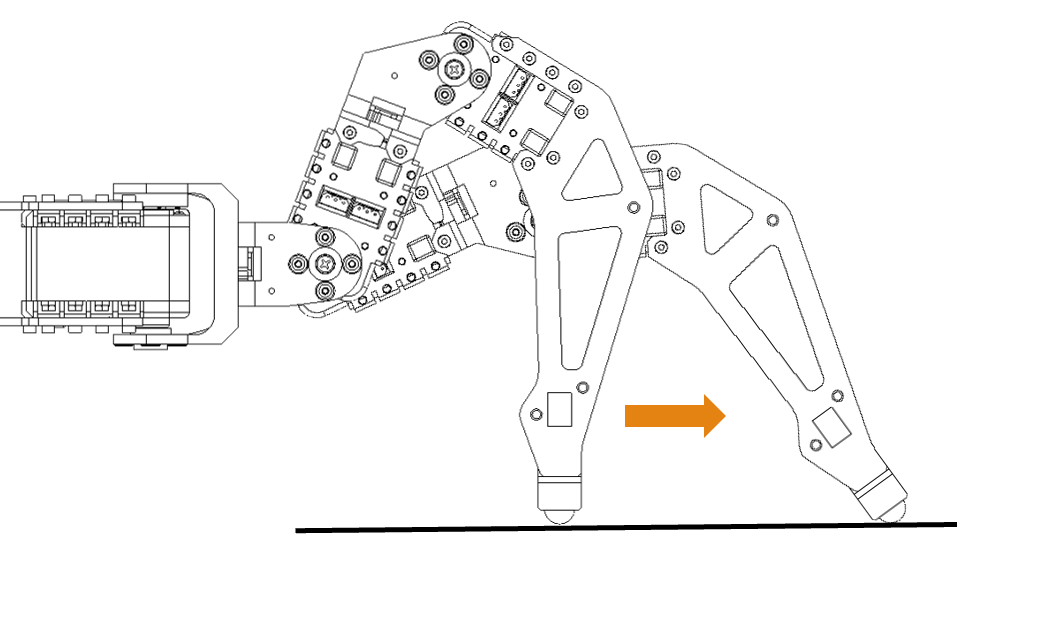
\includegraphics[width=0.48\columnwidth]{figure/chapter2/leg_range.png}}
  \hspace{0.04\columnwidth}
  \subfigure[Determination of the Maximum Radius]{%
  \label{fig:leg_range_b}
  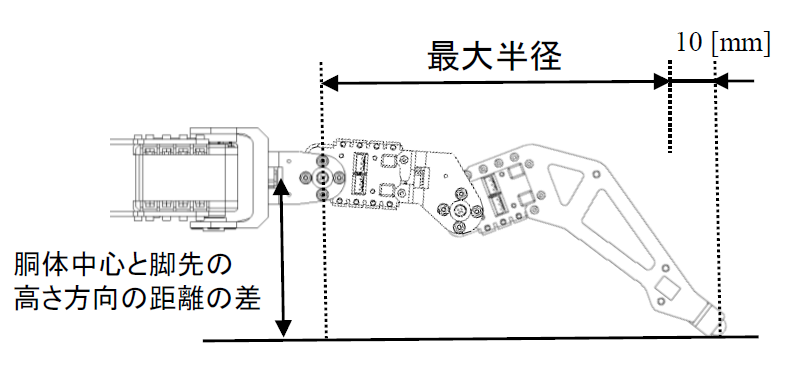
\includegraphics[width=0.48\columnwidth]{figure/chapter2/max_leg_range.png}}
  \caption{Comparelegmodel}
  \label{fig:leg_range}
\end{figure}

\subsection{脚軌道生成の失敗}
先行研究ではグラフの階層構造化および脚軌道生成の分離によって,実時間内の計算が可能になった.
しかし,実際に実機を用いて歩行実験を行ったところ,低頻度ではあるが脚軌道生成に失敗することがあった.
失敗の原因として,脚の可動範囲に近似的な値を用いていることがあげられる.
近似的な脚の可動範囲の境界近くは,実際には脚の可動範囲外であるが,
近似的な値を用いているために脚の可動範囲内と判定されてしまっている領域があると考えられる.
そのため,脚軌道や脚の接地点が脚の可動範囲外になってしまい,脚軌道生成に失敗することがあると考えられる.

% 予備実験の章
\section{歩行シミュレーションによる脚軌道生成失敗時の脚先位置の特定}

\subsection{シミュレーション実験の目的}
先行研究では脚軌道生成の失敗による動作の停止が報告された上,
その原因は脚先が脚の可動範囲の外を通ることによるものであると考察されてきた.
しかし,具体的に脚先がどのような位置になると脚軌道生成が失敗するのかは明らかにされていなかった.
そのため予備実験として,波東らの研究\cite{Hato_Graph_search}の実機試験と同じ条件で歩行シミュレーション実験を行い,
ロボットの脚軌道を確認することで,脚軌道生成失敗の原因を特定することにした.

\subsection{シミュレーションの条件}
本研究室ではロボットの動作のシミュレーションを行うためのシミュレーターソフトウェアを自作し,
シミュレーション実験を行ってきた.
本論文でも同様に,シミュレーション実験に自作のシミュレーターソフトウェアを用いた.

シミュレーターはC++で記述されており,WindowsAPIを用いてGUIを実装し,ロボットを表示している.
また,GUIの表示のプログラムをより簡単に記述するため,
ゲームプログラミングに用いられるライブラリのDxLib\cite{Dxlib_Web}を用いている.
シミュレーターは物理演算を行っておらず,トルク不足や摩擦,脚先の滑りによるずれを考慮していない.
そのため,ロボットのアクチュエータは無限のトルクを持ち,脚先は滑りなく接地するものと仮定している.
本来これらのパラメータを考慮すべきではあるが,
本研究においては歩容パターン生成によって得られた脚接地点に脚先を届かせることが可能であるか確認することが目的であるため,
これらのパラメータは考慮しないこととしている.

\subsubsection{シミュレーションの計算環境}
シミュレーションの計算環境は\tableref{tab:simulation_env}に示したとおりである.

% 計算環境の表
\begin{table}[htbp]
	\caption{Simulation Environment}
	\label{tab:simulation_env}
	\begin{center}
   	\begin{tabular}{|c||c|} \hline
      CPU & 11thGen Intel Core(TM) i5-11400  \\ \hline
      RAM & 32.0GB  \\ \hline
      OS & Windows 11 Home  \\ \hline
      開発環境 & Visual Studio 2022 Community  \\ \hline
      使用言語 & C++20  \\ \hline
    \end{tabular}
  \end{center}
\end{table}

\subsubsection{モデルとするロボット}
モデルとするロボットは,Trossen Robotics社のPhantomX Mark I\hspace{-1.2pt}I \cite{cita:phantom_x_mark_2}
(以下PhantomX)とする.
PhantomX(\figref{fig:phantomx_mk2})は6脚ロボットであり,各脚に3つのアクチュエータを持つ.
また,関節配置は脚の付け根からヨー・ピッチ・ピッチの順である.

\begin{figure}[htbp]
  \begin{center}
    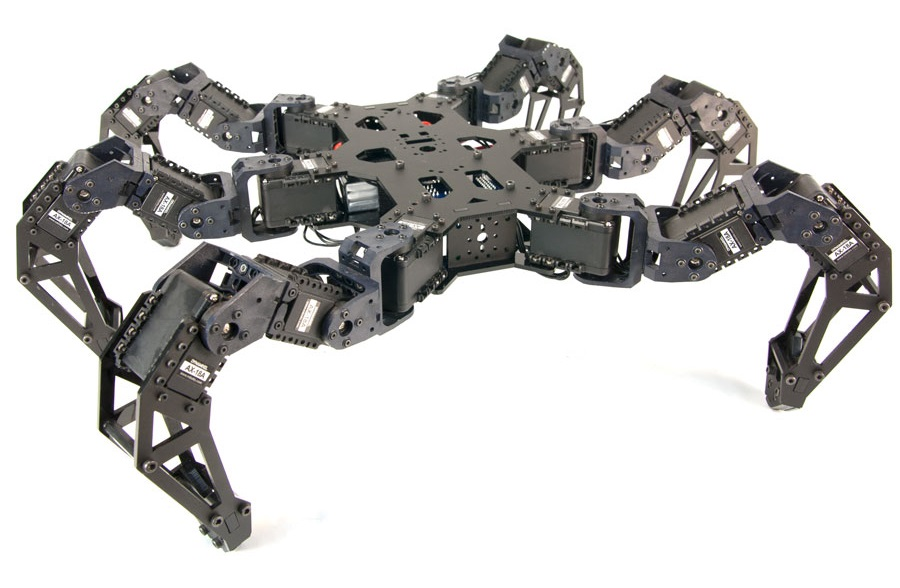
\includegraphics[width=45mm, clip]{figure/chapter2/phantomx_mk2.jpg}
    \caption{PhantomX Mark I\hspace{-1.2pt}I}
    \label{fig:phantomx_mk2} % chktex 24
  \end{center}
\end{figure}

\subsubsection{歩行する地形}
歩行する地形を\figref{fig:terrain}に示す.
地形は5種類あり,それぞれ平地,上り段差,下り段差,上り斜面,下り斜面である.
実機試験の条件に合わせ,段差は上り,下りともに高さが$100 [mm]$とし,
斜面は上り,下りともに角度が$15 [deg]$とした.

\subsection{シミュレーションの結果}
以下の図に脚軌道生成失敗時の脚先の座標を示す.

\subsection{脚軌道生成に失敗する原因の考察}

% 常に脚軌道生成が可能な自由歩容パターン生成手法の検討の章
\section{常に脚軌道生成が可能な自由歩容パターン生成手法の検討}
常に脚軌道生成を可能にするためには,近似された脚可動範囲を適切に設定する必要がある.


% 再評価手法の提案の章
\section{歩容パターンの再評価手法}

